\begin{figure*}[t]
    \centering
    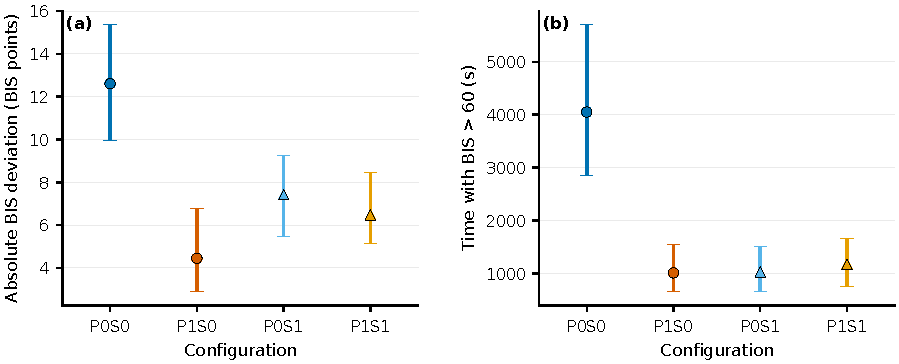
\includegraphics[width=\textwidth]{figures/main_control_performance.pdf}
    \caption{Final sealed-test control performance for the four evaluated
    preprocessing--state configurations. Points show case-level medians and error
    bars show case-level interquartile ranges across 490 evaluation cases. Lower
    values are better for both mean absolute BIS deviation and time with BIS
    greater than 60. Color encodes the preprocessing profile and marker shape
    encodes the state representation.}
    \label{fig:main-control-performance}
\end{figure*}

\begin{figure*}[t]
    \centering
    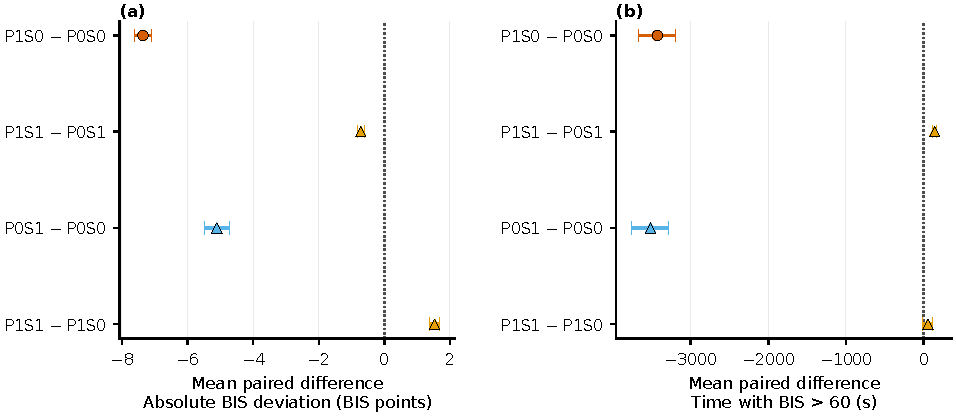
\includegraphics[width=\textwidth]{figures/paired_control_effects.pdf}
    \caption{Prespecified subject-level paired contrasts on the sealed test set
    ($n=483$ subjects). Points are mean within-subject differences and error bars
    are 95\% paired-bootstrap confidence intervals based on 2,000 replicates; the
    dotted line denotes no difference. Negative values favor the first-named
    configuration in each contrast, because lower values indicate better
    control.}
    \label{fig:paired-control-effects}
\end{figure*}
